Como se ha comentado anteriormente, el primer paso para monitorizar los niveles de agua tritiada es detectar los electrones que se producen en la desintegración $\beta^-$ del tritio (ecuación  $\eqref{desintegraciontritio}$). Para ello, se utilizó  fibras centelleadoras existentes en el mercado, seleccionadas por sus características favorables para nuestro experimento~\cite{Alberto}.  Se determinó que las fibras BCF-12 de Saint Gobain eran las que mejor se ajustaban a los requisitos del experimento. 


\begin{figure}[hbtp]
\centering
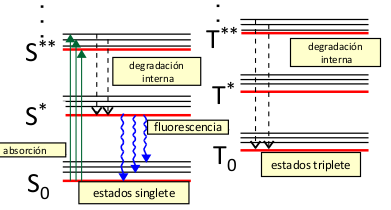
\includegraphics[scale=0.7]{EsquemaNivelesFIbras.png}
\caption{Esquema de niveles energéticos de un material centelleador~\cite{asignatura}\label{Esquemafibras}
}
\end{figure}


Un plástico centelleador esta dopado con  materiales luminiscentes cuyas moléculas poseen  niveles energéticos similares a los de la figura \ref{Esquemafibras},
donde los estados $S$ representan singletes y los estados $T$ tripletes. Cuando la radiación ionizante, en nuestro caso los electrones procedentes del tritio,  atraviesan el centelleador, sus moléculas absorben la energía, produciéndose una excitación de las mismas. 
A continuación éstas se desexcitan, en primer lugar desde niveles superiores hasta el nivel $S*$ o $T_0$ por degradación interna (en un tiempo del orden del $\pico\second$) y seguidamente del S* hasta $S_0$ (en un tiempo del orden del $\nano\second$). En esta segunda desexcitación se emiten fotones, cuya longitud de onda puede ir desde el ultravioleta hasta el infrarrojo $[100-800 \nano\meter]$, dependiendo de la distancia existente entre estos niveles energéticos. La emisión de estos fotones se conoce con el nombre de  fluorescencia, y es el mecanismo que produce la señal de respuesta de un material centelleador orgánico(Fig. $\ref{Espectros}$).
Las fibras centelleadoras son transparentes a los fotones que se encuentran en la longitud de onda de su emisión, ya que, de lo contrario, tendríamos una reabsorción de los fotones emitidos antes de ser detectados por el fotosensor, inhibiendo la señal.

Los materiales centelleadoras presentan una muy buena linealidad con la energía de la radiación incidente a partir de una energía mínima, que determina la sensibilidad del material centelleador. Teniendo en cuenta que los SiPM también presentan una muy buena linealidad con la señal recibida, esperamos obtener una respuesta de nuestro detector que presente una buena linealidad con la energía de la señal.

Por lo general, los plásticos centelleadores producen señales bastante rápidas en comparación con otros tipos de detectores. Utilizamos fibras centelleadoras orgánicas, ya que estas son 2 o 3 órdenes de magnitud más rápidas que las inorgánicas,  en concreto, las fibras que utilizaremos presentan un tiempo de atenuación de $3.2~\nano\second$~\cite{datasheet}. Poseen un índice de refracción de $n=1.6$, parámetro fundamental a la hora de transportar eficientemente la luz.

Las fibras centelleadoras elegidas deben de producir el mayor número de fotones  posible por unidad de energía para poder tener una señal lo mayor posible. Las fibras BCF-12 producen unos  $8000$ fotones por $\MeV$ de la radiación incidente y tienen una eficiencia de fotodetección  del $3.4\%$~\cite{datasheet}.

Para manipular las fibras se vio necesario la utilización de guantes de látex, ya que el contacto con las manos  las ensuciaban, afectando a  la propagación de la luz.

\begin{figure}[htb]
\centering
{
%\subfloat[Espectro de emisión]
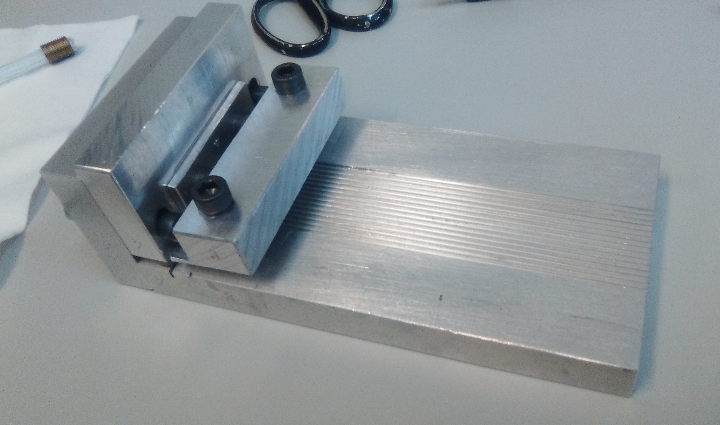
\includegraphics[scale=0.25]{Guillotina1.png} 
}
{
%\subfloat[Espectro de emisión]
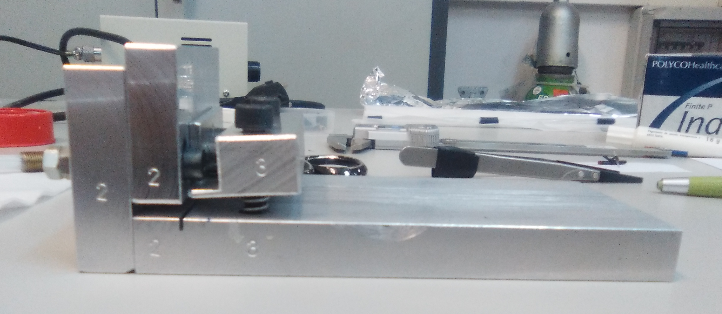
\includegraphics[scale=0.33]{Guillotina2.png} 
}
\caption{Guillotina\label{Guillotina}}
\end{figure} 


Para poder cortar las fibras centelleadoras de forma ópticamente aceptable, se diseñó y construyó una guillotina adecuada en los talleres del IFIC~\cite{Alberto,anguloytiempo, dependencias, tesisfibras}, la cual se muestra en la figura~\ref{Guillotina}.
En la parte derecha  de la figura se puede observar que la guillotina está constituida de dos piezas independientes (marcadas con los números 2 y 3), las cuales están suspendidas por muelles. Para sujetar y cortar  las fibras, hay que pulsar  secuencialmente las piezas 3 y 2. 
La guillotina dispone de 14 rieles cuadrados, los cuales sirven para sujetar cada una de las fibras y, así, obtener un corte limpio y perpendicular. Aunque la guillotina tiene la posibilidad de realizar cortes simultáneos sobre varias fibras centelleadoras, siempre se realizaron cortes sobre una única fibra. De esta forma asegurábamos un mejor acabado.

Se estuvo probando con varios tipos de cuchilla (de distinto grosor y tamaño),  y se obtuvo que una cuchilla típica de afeitar era adecuada. Hay que tener en cuenta que, para un corte más efectivo, se introdujo en la disposición de la cuchilla una ligera inclinación~\cite{Alberto, anguloytiempo}. 

En la figura~\ref{Pulido} izquierda, obtenida  con ayuda de un microscopio, se puede ver  la cara de una fibra óptica con clad recién cortada. En ésta  figura podemos apreciar que, aunque presenta una acabado realmente bueno (sin roturas ni deformaciones), la cara de la fibra se encuentra ligeramente dañada,  lo que afecta a la transmisión de la luz. La forma de subsanar este problema fue pulir cada una de las caras de las fibras. En la parte derecha de la misma figura podemos observar una foto con la misma fibra tras el proceso de pulido. Podemos comprobar que el simple hecho de pulir las caras de las fibras nos permite mejorar sensiblemente el  acabado óptico~\cite{Alberto, manual}.
\begin{figure}[htb]
\centering
{
%\subfloat[Espectro de emisión]
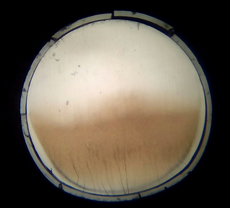
\includegraphics[scale=0.6]{SinPulir.png} 
}
{
%\subfloat[Espectro de emisión]
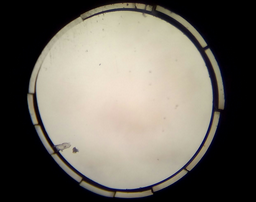
\includegraphics[scale=0.6]{Pulida.png} 
}
\caption{Cara fibras\label{Pulido}}
\end{figure} 
Hay que notar en la figura que el clad está roto. Se vio que esto era una característica inevitable del proceso de cortado. Sin embargo, pudo observarse que la ruptura únicamente se encontraba en el extremo final de la fibra, por lo que  la utilización de grasa óptica  (Saint-Gobain, BC-360) para acoplar ésta al fotosensor solucionaba el problema.  De todas formas, las fibras centelleadoras empleadas en este trabajo no tienen clad, por lo que no les afecta este problema. 
%La grasa óptica utilizada posee un índice de refracción de 1.465, parecido al de las fibras utilizadas, 1.49.

Seguidamente, con las fibras ya cortadas, se utilizó un pegamento óptico (también de  la marca Saint Gobain), especialmente diseñado para materiales centelleadores, para pegarlas entre ellas y obtener, de esta forma, un haz de fibras. Para que su acabado fuese suficientemente rígido se introdujo cada uno de los extremos del haz de fibras en un anillo metálico, mostrado en la figura~\ref{Arofibra}. En la figura~$\ref{Arofibra}$ derecha puede observarse que los anillos disponen  de una tuerca, la cual se utiliza para una completa sujeción al prototipo.
Finalmente, cuando se había secado el pegamento, volvíamos a pulir cada una de las caras del haz de fibras con el objetivo de obtener una cara completamente plana (todas las fibras al mismo nivel) para obtener un  acoplamiento óptimo con el fotosensor (ya sea SiPM o PMT). En la figura~$\ref{Bunch}$ podemos observar un  haz de fibras totalmente acabado.


\begin{figure}[htb]
\centering
{
%\subfloat[Espectro de emisión]
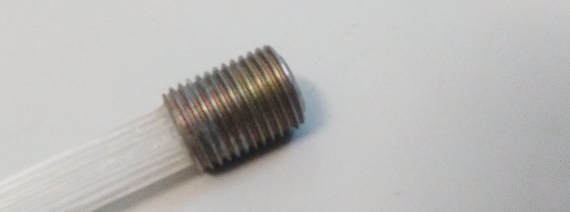
\includegraphics[scale=0.4]{arometalico.png} 
}
{
%\subfloat[Espectro de emisión]
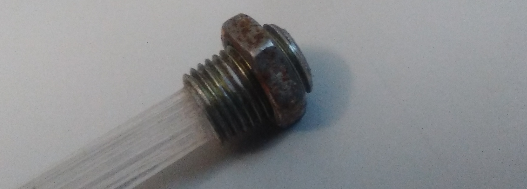
\includegraphics[scale=0.4]{arometalicoconrosca.png} 
}
\caption{Aro metálico\label{Arofibra}}
\end{figure} 




\begin{figure}[htb]
\centering
{
%\subfloat[Espectro de emisión]
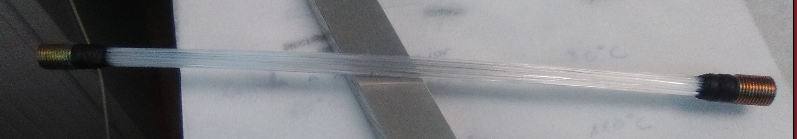
\includegraphics[scale=0.33]{bunchfibras.png} 
}
{
%\subfloat[Espectro de emisión]
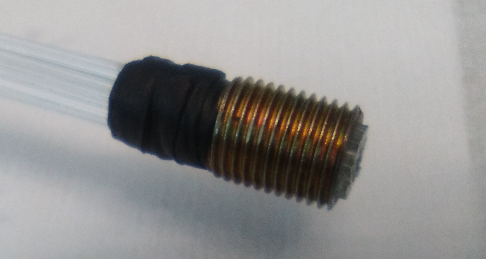
\includegraphics[scale=0.33]{bunchfibras1.png} 
}
\caption{Haz de fibras centelleadoras\label{Bunch}}
\end{figure} 

El haz  construido consiste de $35$ fibras, que es el mayor número de fibras que cabe en el interior del anillo metálico, y tiene una longitud de aproximadamente $25\cm$, extensión acorde con el prototipo. En la figura~\ref{Bunch} derecha, podemos observar la cara final pulida, perfectamente plana. Hay que tener en cuenta que cualquier irregularidad inferior al milímetro en la cara final del haz es subsanada por la grasa óptica empleada para acoplar el haz de fibras al fotosensor.
